\subsubsection{Structure du code}

J'ai repris deux projets différents :

\begin{itemize}
    \item \textbf{Bike Accessibility}, comprenant l'implémentation du modèle exact détaillé dans la section \ref{modelesexacts} (seulement les critères d'optimisation \ref{criterepoi} et \ref{criterepopu} de \ref{criteresopti}), créé par Tifenn Rault et Emmanuel Néron. Pour résoudre les modèles exacts, nous utilisons CPLEX, un outil informatique d'optimisation commercialisé par IBM \cite{cplex}. Le projet Bike Accessibility est écrit en C++, et utilise la technologie Concert pour utiliser CPLEX \cite{concert}.

    \item \textbf{Chemins Equitables}, une application de visualisation des réseaux cyclables créée par Alaâ Chakori Semmane et Jérôme Lécuyer en 2024. Cette application est écrite en Java et en Python.
\end{itemize}

\subsubsection{Fichiers de données}\label{sect:fichiersdonnees}

Pour récupérer les données décrites section \ref{sect:modelisation}, nous utilisons, pour un graphe, 4 fichiers \verb|.csv| :

\begin{itemize}
    \item \verb|<nom_graphe>_noeuds.csv|, qui contient l'identifiant de chaque noeud du graphe.
    \item \verb|<nom_graphe>_arcs.csv|, qui contient pour chaque arc du graphe son noeud de départ, son noeud d'arrivée, la distance de l'arc et son danger. Le ratio $\fFrac{\text{danger}}{\text{distance}}$ est ce qui donne la colonne facteur de la table \ref{table:lts_tours}.
    \item \verb|<nom_graphe>_filosofi.csv|, contenant pour chaque carreau filosofi son identifiant, son noeud délégué, et diverses informations socio-démographiques.
    \item \verb|<nom_graphe>_poi.csv|, contenant l'identifiant de chaque POI, le noeud du graphe auquel il est associé, et ses tags OpenStreetMap (qui nous donnent diverses informations sur ce POI). 
    % Les fichiers POI utilisés sont toujours ceux issus du filtre def_90 machin, on refiltre dans le parser.  \textcolor{red}{Cela évite d'avoir des problèmes avec le parser}
\end{itemize}

Ce sont les fichiers de données qui étaient déjà utilisés dans le projet Bike Accessibility, j'ai continué de travailler avec eux. 

\subsubsection{Modèles exacts}\label{sect:prog_modelesexacts}

Il a d'abord fallu apporter des modifications au modèle exact commencé dans le projet Bike Accessibility, pour qu'il donne les résultats attendus.

Dans ce même projet, j'ai créé un deuxième modèle exact, optimisant sur la même visibilité que les heuristiques (la visibilité PCC). L'objectif de ce modèle exact était de pouvoir quantifier l'efficacité des heuristiques. 

% Vu que la visibilité de ces deux modèles n'est pas la même, la valeur objective retournée n'est pas la même. En effet, le modèle exact sur la visibilité réduite prend en compte seulement certains chemins parmi tous les chemins potentiels (puisque des arêtes sont amputées au modèle), donc la valeur objective sur la visibilité réduite est moins bonne que la valeur objective sur la visibilité exacte, pour le même graphe avec les mêmes arcs modifiés. 

Dans le modèle exact sur la visibilité PCC, des POI sont trouvés par "accident" : certains chemins entre un noeud délégué et un POI ne sont pas visibles par cette visibilité, puisque certaines arêtes sont amputées au modèle. Donc, lorsqu'on recalcule manuellement le nombre de POI à présent accessibles, ils sont davantage que la valeur objective (\emph{Objective Value}, OV) retournée par ce modèle. La table \ref{tab:nbppoi} montre l'ampleur de ce phénomène pour différentes instances.

Lorsqu'on compare les valeurs objectives des modèles exacts pour ces deux visibilités, il faut prendre en compte ce biais. Donc pour comparer les valeurs objectives des deux modèles exacts, j'ai recodé le calcul de la valeur objective avec la visibilité exacte, ainsi que le calcul de la valeur objective sur la visibilité PCC (appelées OV exacte et OV PCC respectivement).

J'ai implémenté les fonctions objectives cités en \ref{enum:function_obj} pour chacun de ces modèles exacts.

\subsubsection{Heuristiques}

J'ai aussi implémenté les heuristiques décrites en section \ref{sect:heuristiquesopt}, dans le projet Bike Accessibility, en C++. 

Les heuristiques sur le nombre de POI (prenant en compte ou non le nombre de personnes impactées) sont implémentées dans une seule classe, appelée \verb|HeuristicPCC|, et l'heuristique sur la diversité de POI est implémentée dans la classe \verb|HeuristicDiversity|.

Dans les fonctions objectives section \ref{enum:function_obj}, nous pouvons observer que symétriquement aux fonctions objectives 1 et 2, nous pouvons créer la fonction objective 
$$\Maximize \sum_{z \in \mathcal{Z} } \sum_{c \in \mathcal{C}} cat_c^z w_z,$$ une extension naturelle de la fonction objective 3 où l'on prendrait en compte le nombre de personnes impactées.

Je n'ai pas eu le temps de faire de tests sur cette fonction objective (bien que je l'ai implémentée), et je n'ai pas codé d'heuristiques cherchant à imiter son comportement (bien que j'ai aussi pensé à cette amélioration potentielle et que j'ai structuré \verb|HeuristicDiversity| dans l'optique qu'elle soit facilement implémentable).

\subsubsection{Fichiers résultats et génération de tables}

Chaque modèle produisait des fichiers résultats contenant diverses informations sur l'optimisation effectuée, comme le temps pris, les valeurs objectives au début et à la fin de l'optimisation, sur la visibilité exacte et sur la visibilité PCC (notons que la valeur objective \emph{initiale} est aussi différente si elle est calculée avec la visibilité exacte ou réduite, parce qu'il peut initialement avoir un chemin entre un carreau et un POI qui ne soit pas un PCC), les arcs aménagés, etc.

J'ai créé des scripts Python permettant de générer facilement des tables de résultats en parsant les fichiers résultats. 


\subsubsection{Visualisation de l'équité d'un réseau cyclable}

\paragraph{Intérêt de la visualisation}

L'application Chemins Equitables permettait déjà de visualiser sous forme de carte le contenu des quatre fichiers \verb|.csv| décrit en section \ref{sect:fichiersdonnees}.

L'intérêt d'une telle application est de pouvoir communiquer avec les acteurs du projet qui s'occupent de l'aspect cartographie. Je leur ai fourni mes cartes, pour qu'ils puissent avoir un avis sur la pertinence des résultats trouvés.Cette application est aussi pratique pour contrôler visuellement les résultats d'optimisation trouvés.

\paragraph{Fonctionnement}

Dans cette application, il y a deux parties :

\begin{itemize}
    \item Des scripts de génération de données. A partir de deux fichiers \verb|.csv| donnant des informations sur les arcs et noeuds du graphe (venant d'instances réelles), l'application Chemins Equitables génère les fichiers \verb|.csv| Filosofi et POI associés grâce aux données de l'INSEE et d'OpenStreetMap. C'est donc ici que les 4 fichiers \verb|.csv| sur lesquels l'optimisation s'effectue sont générés.
    \item Un visualisateur, qui permet de créer des cartes à partir d'un jeu de données créé précédemment. 
\end{itemize}

Cela donne une carte ressemblant à la figure \ref{figu:fondettes}.

\begin{figure}[H]
    \centering
    \begin{subfigure}[t]{0.45\textwidth}
        \centering
        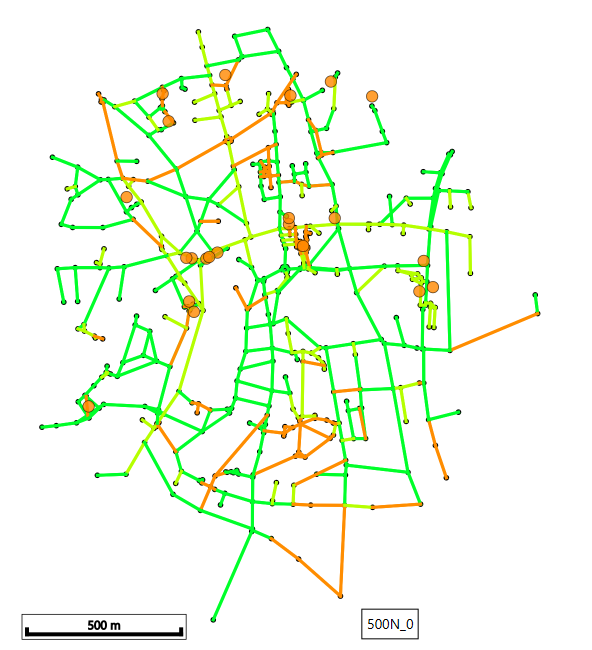
\includegraphics[width=0.7\linewidth]{500N_0_ajusted.png}
        \caption{Carte obtenue en chargeant un certain jeu de données. On remarque que la géométrie des tronçons n'est pas conservée.}
    \end{subfigure}
    \hfill
    \begin{subfigure}[t]{0.45\textwidth}
        \centering
        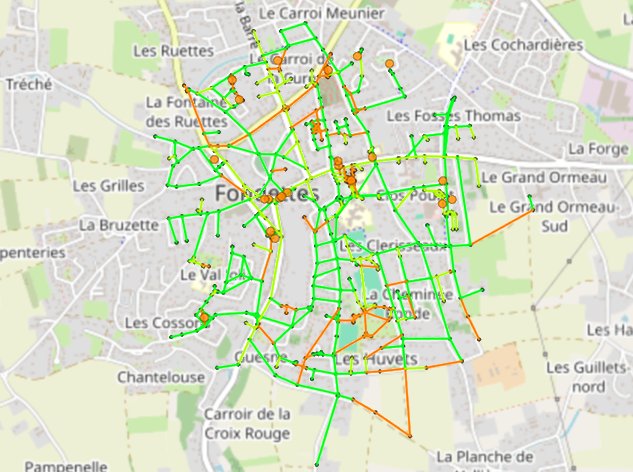
\includegraphics[width=1\linewidth]{superposition_fondettes_zoom.png}
        \caption{En superposant la carte obtenue avec une carte plus détaillée. Il s'agit de la ville de Fondettes, à proximité de Tours.}
    \end{subfigure}
    \hfill
    \caption{}
    \label{figu:fondettes}
\end{figure}

La légende du danger des arcs est la suivante :
\begin{itemize}
    \item Vert : LTS 1,
    \item Jaune : LTS 2,
    \item Orange : LTS 3,
    \item Rouge : LTS 4.
\end{itemize}

\paragraph{Modifications apportées :}\label{sect:modifs_chemins_eq}

L'application Chemins Equitables en l'état permettait de visualiser un réseau cyclable pré-optimisation. J'ai dû modifier cette application pour qu'elle prenne en charge les données que j'ai créés. Les modifications que j'ai faites sont les suivantes :

\begin{itemize}
    \item Création d'un nouveau jeu de données post-optimisation : il s'agissait de créer quatre nouveaux fichiers \verb|.csv| compatibles avec le visualisateur. J'ai créé un nouveau script copiant les deux fichiers donnant des informations sur les arcs et noeuds du graphe de l'instance sur laquelle l'optimisation a été faite, puis j'ai modifié le fichier donnant des informations sur les arcs pour modifier le danger des arcs aménagés. Les quatre fichiers \verb|.csv| sont ensuite générés en utilisant les mêmes scripts.
    \\
    Par aménager un arc, on entend mettre son niveau LTS au minimum, donc à 1. C'est à dire que son danger, dans le fichier \verb|.csv|, devrait valoir sa distance. Pour des raisons de simplification pour le visualisateur, \textbf{j'ai mis le niveau LTS des arcs aménagés à 0} dans le fichier \verb|<nom_graphe>_arcs.csv|. Ce choix a été fait pour que je puisse passer davantage de temps sur la partie optimisation du problème, ce sur quoi mon stage est centré, mais l'idéal aurait été de rajouter un nouvel attribut de classe aux arcs pour le visualisateur.
    \\
    Par rapport aux fichiers POI, la façon dont ils sont générés nécessite de changer dans le \verb|Makefile| le filtre des POI en fonction de l'optimisation choisie, pour être cohérente avec celle-ci. Par exemple, si l'on a optimisé seulement sur les POI de certaines catégories, pour des raisons de lisibilité, l'on ne veut pas que dans le jeu de données des POI sur lesquels on n'a pas optimisé soit présents.
    \item Programmation de nouveaux PM : il a fallu que je programme de nouveaux PM, en particuler ceux associé à chaque critères d'optimisation, de sorte à quantifier le avant-après de chaque optimisation (ainsi que la qualité des différents modèles d'optimisation). 
    \item Traitement des arcs aménagés par le visualisateur et par les algorithmes de calcul de PM : mettre à 0 le danger d'un arc aménagé m'a permis de facilement modifier sa couleur pour qu'ils ressortent sur une carte, sans changer en profondeur la structure du code. J'ai aussi dû modifier certains algorithmes, pour qu'ils traitent les arcs de LTS 0 comme des arcs de LTS 1, pour préserver le bon fonctionnement des fonctionnalités qui étaient déjà implémentées dans l'application.
    \item Suppression des trois arcs stressants autorisés : pour des questions de réalisme, dans le calcul des algorithmes de recherche de chemins (qui interviennent notamment dans le calcul des PM), Jérôme et Alaâ se sont autorisés à emprunter trois arcs stressants, c'est à dire avec un niveau LTS supérieur au niveau LTS maximal autorisé. J'ai supprimé cette fonctionnalité (je l'ai commentée dans le code), parce qu'on ne s'autorise pas ça dans la partie optimisation, dans le projet Bike Accessibility. Mais idéalement, ça pourrait être quelque chose intégré aussi dans l'optimisation.
    \item Les arcs à aménager sont affichés en rose. Sur les cartes, entre deux noeuds, les arcs dans les deux sens sont superposés. Il est donc possible qu'un arc soit caché par un autre arc. J'aurais souhaité faire en sorte que les arcs aménagés aient une priorité supérieure aux autres arcs, pour qu'ils soient toujours clairement visibles. Je n'ai malheureusement pas eu le temps de me pencher sur cet aspect, et j'ai seulement rendu ces arcs plus épais pour qu'ils soient toujours un minimum visibles.
\end{itemize}

Dans le fichier \verb|<nom_graphe>_filosofi.csv|, certains carreaux ne comportent pas d'informations socio-démographiques. Sur le projet Bike Accessibility, nous ne nous occupons pas de ces carreaux, ils ne sont pas rattachés aux modèles d'optimisation. Sur le projet Chemins Equitables, ces carreaux sont quand même pris en compte : les PM sont quand même calculés sur ces carreaux. J'aurais voulu griser ces carreaux, de sorte à ce que ça soit clair sur quels carreaux l'optisation s'est effectuée, mais je n'ai pas eu le temps de faire ça.